% TikZ code representing basic logic gates (AND, OR, NOT) and their corresponding quadratic equations over F_2.

\usetikzlibrary{arrows.meta}

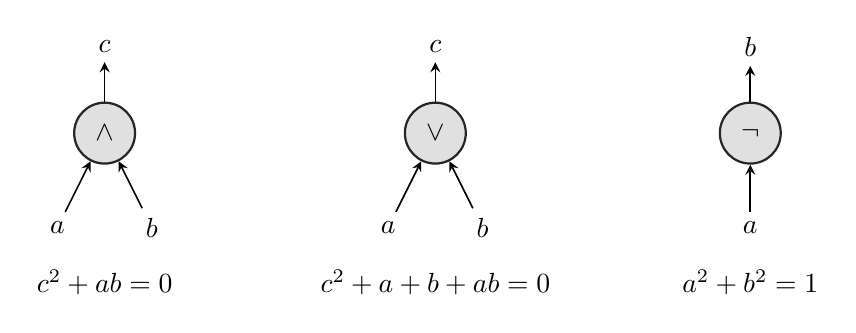
\begin{tikzpicture}[
    scale=1.0,
    gate/.style={circle, draw=black!85, fill=black!12, thick, minimum size=22pt, inner sep=0pt},
    arrow/.style={->, >=stealth, semithick}
]

    % --- Porta AND ---
    \begin{scope}[xshift=0cm]
        % Inputs
        \node (a1) at (-0.6, 0) {$a$};
        \node (b1) at (0.6, 0) {$b$};
        % Gate
        \node[gate] (and) at (0, 1.2) {$\land$};
        % Output
        \node (c1) at (0, 2.3) {$c$};
        
        \draw[arrow] (a1) -- (and);
        \draw[arrow] (b1) -- (and);
        \draw[arrow] (and) -- (c1);
        
        \node at (0, -0.7) {$c^2 + ab = 0$};
    \end{scope}

    % --- Porta OR ---
    \begin{scope}[xshift=4.2cm]
        % Inputs
        \node (a2) at (-0.6, 0) {$a$};
        \node (b2) at (0.6, 0) {$b$};
        % Gate
        \node[gate] (or) at (0, 1.2) {$\lor$};
        % Output
        \node (c2) at (0, 2.3) {$c$};
        
        \draw[arrow] (a2) -- (or);
        \draw[arrow] (b2) -- (or);
        \draw[arrow] (or) -- (c2);
        
        \node at (0, -0.7) {$c^2 + a + b + ab = 0$};
    \end{scope}

    % --- Porta NOT ---
    \begin{scope}[xshift=8.2cm]
        % Input
        \node (a3) at (0, 0) {$a$};
        % Gate
        \node[gate] (not) at (0, 1.2) {$\neg$};
        % Output
        \node (b3) at (0, 2.3) {$b$};
        
        \draw[arrow] (a3) -- (not);
        \draw[arrow] (not) -- (b3);
        
        \node at (0, -0.7) {$a^2 + b^2 = 1$};
    \end{scope}

\end{tikzpicture}
